
\section*{Appendix A: proof of Theorem 2}
We provide the proof for resource inequality in the Theorem 2 and consequently the in-equivalence of the signaling $(n\rightarrow 1)$ RB and the $B_n$-box. We give the proof in two parts: 
\begin{enumerate}
\item We shall show that if the bit of communication is not used to send the output of Alice's RB $A$ then the $B_n$-box cannot be obtained.
\item If the bit of communication is used to send $A$ and the $B_n$-box is obtained, then the capacity of obtainable channel $\Lambda$ is upper bounded by $\frac{1}{n}$ bit. 
\end{enumerate}
\subsection*{Part I}
The part I says that if we do not input $A$ to $A'$ then the $B_n$-box cannot be obtained.\\
Let us denote $m$ for the one-bit message to be communicated to Bob. The goal is to obtain perfect $B_n$ correlations i.e. $Y=X\oplus x_y$ in any case, $m=0$ or $1$. Bob's output for any given $m$ depends on RAC's settings on Bob's side: $Y=Y(b,A',B)$. For any fixed $m=m_0$ there are two possible cases $A'=A$ and $A\neq A'$. In the first case $B_n$ correlations are obtained using by processing a perfect RAC. But in the case $A'\neq A$ the signaling $(n \rightarrow 1)$ RB outputs a random $B$ which does not depend on the work of RAC. Hence $Y$ can be obtained solely from processing of $y$ i.e. $Y=Y(y)$. Since we want to obtain perfect $B_n$ correlations $Y(y=0)=X$ and $Y(y\neq 0)=X\oplus x_y$. By adding  $Y(y=0)$ and $Y(y\neq 0)$, Bob can compute $x_y$. We therefore obtain, that in the case $A'\neq A$, the value of $x_y$ must be known to Bob.\\
The signaling $(n\rightarrow 1)$ RB is no-signaling from Bob to Alice. For $y\in \{0,1,..n-1\}$ and $n>2$, Alice cannot know in advance the value of $y$ in order to send $m=x_y$. These leaves only one option to send $A$ which shall be dealt with in the next part $\blacksquare$.
\subsection*{Part II}
We will show using information theoretic tools, that if the signaling $(n\rightarrow 1)$ RB considered in Theorem 2 supplemented with one bit of communication is to reproduce exactly the $B_n$-box and some channel, then the mutual information of the channel must be bounded by $\frac{1}{n}$ bit (assuming that Alice's output of the RB $A$ will be inserted directly into as Bob's second input to the RB i.e. $A'=A$). \\
\textit{Assumptions:} Alice is given variables $x_1,x_2,..x_{n-1}$ and z. Bob is given variable $y\in \{0,1,..n-1\}$. Both are given access to common variable s such that $x_1,x_2,..x_{n-1},z,y,s$ are mutually independent. Alice generates $A$ from $x_1,x_2,..x_{n-1},z,s$ and inputs $a_0,a_1,..a_{n-1}$ to the RAC. Bob generates $b$ from $y,s$ and inputs it into the RAC. These strategies result in shared joint probability distribution $p(x_1,x_2,..x_{n-1},z,y,s,b,A',A,B)$, where $B=a_b$ is obtained from the $(n\rightarrow 1)$ RAC on Bob's side, and $Y$ is generated out of $b,B,s,y$ by Bob. 
First we shall express the Theorem 2 in other words. Under Assumptions 1, if variables $x_1,x_2,..x_{n-1},y,A,B$ perfectly reproduce $B_n$ correlations, there holds:
\begin{equation}
I(z:B,b,y,s)\leq \frac{1}{n}
\end{equation}
where $z$ is the message that Alice sends to Bobs.
We shall prove the above in two parts:
\begin{enumerate}
\item First, we shall use entropies and correlations to state the fact that in order to simulate the $B_n$-box Bob has to guess perfectly $X$ when $y=0$ and $x_y\oplus X$ when $y\neq 0$. 
\item Second, we shall show that it is impossible to send more than 1 bit through a channel with 1 bit capacity. As in our case Alice would like to send both $x_1$ and $z$ which bounds Bob's possible information gain about $z$. 
\end{enumerate}
\begin{mydef2}
Under Assumptions 1, if the variables $(x_1,x_2,x_3..x_{n-1},y,A,B)$ simulate perfectly $B_n$ correlations, there holds:
\begin{equation}
I(B:X|b,s,y= 0)=H(X|b,s,y=0)
\end{equation}
\begin{equation}
I(B:X\oplus x_y|b,s,y\neq 0)=H(X\oplus x_y|b,s,y\neq0)
\end{equation}
\end{mydef2}
In order to reproduce the $B_n$-correlations given $y=0$, Bob should perfectly guess $X$, whereas given $y\neq 0$ he should perfectly guess $X\oplus x_y$. 
This implies that there must be $\max_j[p(a=j|B=l,b=k,y=0,s=i)]=1$. Then for $y=0$ the values of variables $B,b,s$ should determine uniquely the value of $X$;, i.e. $H(X|B,b,s,y=0)=0$. In such a case, $I(X:B|b,s,y=0)=H(X|b,s,y=0)$. Analogously, we obtain $I(X\oplus x_n:B|b,s,y\neq 0)=H(X\oplus x_y|b,s,y\neq0)$. $\blacksquare$ \\
\textit{One cannot send more than one bit through a single-bit wire.} \\
Here, we prove the following Theorem which provides the key argument in the proof of Theorem 2. Namely its shows a tradeoff between Bob's correlations with $X$ and $X\oplus x_y$ (that should be high if he simulates $B_n$ correlations) and his correlations with $z$.
\begin{mydef1}
Under aforementioned assumptions, there holds:
\begin{multline}
 \frac{1}{n}[\sum_{i=1}^{n-1}I(X\oplus x_i:B|b,s,y=i) + I(X:B|b,s,y=0)] +\\ 
I(z:B|b,s,y) \leq \\ 
\frac{1}{n}I(X:X\oplus x_1:X\oplus x_2:..:X\oplus x_{n-1}:z |b,s) 
+H(B|b,s,y)
\end{multline}
\end{mydef1}
In the proof for the above Theorem we use the following fact, which captures that one cannot send reliably $n$ bits ($n>1$) through a single bit wire, unless the bits are correlated.
\begin{mydef2}
For any random variables $S_1,S_2,,..S_n,T,V$ there holds:
\begin{equation}
\sum_{i=1}^n I(S_i:T|V) \leq I(S_1:S_2:..S_n:T|V)
\end{equation}
where $I(S_1:S_2:..S_n:T|V)=\sum_{i=0}^{n}H(S_i|V)+H(T|V)-H(S_1,S_2,..S_n,T|V)$
\end{mydef2}
First we proof the above fact without conditioning. We shall use the following fact recursively. For any random variables $S_i,S_j,T$ it follows directly from strong subadditivity: 
\begin{equation}\label{e33}
H(S_iS_jU)+H(T)\leq H(S_iT) + H(S_jT)
\end{equation}
By expressing mutual information via Shannon entropies, we can rewrite LHS as:
\begin{multline}
nH(T)+\sum_{i=1}^{n}H(S_i)-\sum_{i=1}^{n}H(S_iT)
\end{multline}
Using (\ref{e33}) n-1 times we can upper bound LHS by,
\begin{equation}
H(T)+\sum_{i=1}^{n}H(S_i)-H(S_1,S_2,..S_n,T)\equiv I(S_1:S_2:..S_n:T)
\end{equation}
Which is the desired result without conditioning on $V$. We can now fix $V=v$, and the thesis will hold for conditional distribution $p(S_1,S_2,..S_n,T|V=v)$:
\begin{equation}
\sum_{i=1}^n I(S_i:T|V=v) \leq I(S_1:S_2:..S_n:T|V=v)
\end{equation}
The desired thesis is obtained after multiplying each side by $p(V=v)$, and summing over range of variable $V$. $\blacksquare$ \\
Moving on with the proof of Theorem 7. Let us reformulate LHS and fix s=j:
\begin{multline}
 \frac{1}{n}[\sum_{i=1}^{n-1}I(X\oplus x_i:B|b,s=j,y=i) + I(X:B|b,s=j,y=0)] \\ \nonumber
+I(z:B|b,s=j,y) 
\end{multline}
By decomposing the last term into $n$ terms, which depend on the value of $y$ we obtain:
\begin{multline}
 \frac{1}{n}[\sum_{i=1}^{n-1}(I(X\oplus x_i:B|b,s=j,y=i) + I(z:B|b,s=j,y=i))+ \\
I(X:B|b,s=j,y=0) + I(z:B|b,s=j,y=0)]
\end{multline}
We use Lemma 4 (for $n=2$) pairwise to show that the above quantity is upper bounded by
\begin{multline}\label{e38}
\frac{1}{n}[\sum_{i=1}^{n-1}(I(X\oplus x_i:z|b,s=j,y=i) + \\ I(B:X\oplus x_i,z|b,s=j,y=i))+
I(X:z|b,s=j,y=0) + \\ I(B:X,z|b,s=j,y=0)]
\end{multline}
Observe that $(X\oplus x_i,z|s=j)$ is independent from $(y,b|s=j)$, hence there is $I(X\oplus x_i:z|b,s=j,y=i)=I(X\oplus x_i:z|b,s=j)$ and similarly $I(X:z|b,s=j,y=0)=I(X:z|b,s=j)$. Multiplying both sides these equalities by $p(s=i)$ and summing up over values of $s$ we get $I(X\oplus x_i:z|b,s,y=i)=I(X\oplus x_i:z|b,s)$ and $I(X:z|b,s,y=0)=I(X:z|b,s)$. Applying the same to (\ref{e38}) and using the latter equalities we obtain:
\begin{multline}\label{e38}
\frac{1}{n}[\sum_{i=1}^{n-1}(I(X\oplus x_i:z|b,s) + I(B:X\oplus x_i,z|b,s,y=i))+ \\
I(X:z|b,s) + I(B:X,z|b,s,y=0)]
\end{multline}
So that we can use Lemma 4 to the terms $\sum_{i=1}^{n-1}I(X\oplus x_i:z|b,s)+I(X:z|b,s)$ to obtain:
\begin{multline}
\frac{1}{n}[ I(X:X\oplus x_1:X\oplus x_2:..X\oplus x_{n-1}:z|b,s)+ \\ \sum_{i=1}^{n-1}I(B:X\oplus x_i,z|b,s,y=i)+ \\
 + I(B:X,z|b,s,y=0)]
\end{multline}
The terms $I(B:X\oplus x_i,z|b,s,y=i)$ are bounded by $H(B|b,s,y=i)$. Similarly the term $I(B:X,z|b,s,y=0)$ is bounded by $H(B|b,s,y=0)$ which because of the factor $\frac{1}{n}$ give rise to $H(B|b,s,y)$ and the assertion follows. $\blacksquare$ \\
Finally, we come back to the proof of Theorem 2. We now prove the main result. To this end, we first observe that in fact it is sufficient to show:
\begin{equation} \label{rf}
I(z:B|b,y,s) \leq \frac{1}{n}
\end{equation}
Indeed from the chain rule: $I(z:B,b,s,y)=I(z:y,b,s)+I(z:B|b,y,s)$, but $I(z:y,b,s)=0$ by assumption. Hence we get,
\begin{equation}
I(z:B,b,s,y)=I(z:B|b,y,s) \leq \frac{1}{n}
\end{equation}
which is the desired bound. To show (\ref{rf}), we use Theorem 7 and Lemma 3. From Theorem 7 we have:
\begin{multline}
 \frac{1}{n}[\sum_{i=1}^{n-1}I(X\oplus x_i:B|b,s,y=i) + I(X:B|b,s,y=0)] \\ 
I(z:B|b,s,y) \leq \frac{1}{n}I(X:X\oplus x_1:X\oplus x_2:..:X\oplus x_{n-1} |b,s) \\
+H(B|b,s,y)
\end{multline}
Now using Lemma 3 we get:
\begin{multline}
 \frac{1}{n}[\sum_{i=1}^{n-1}H(X\oplus x_i|b,s,y=i) + H(X|b,s,y=0)] \\ 
I(z:B|b,s,y) \leq \frac{1}{n}[\sum_{i=1}^{n-1}H(X\oplus x_i|b,s)+H(X|b,s)+H(z|b,s)\\-H(X,X\oplus x_1,X\oplus x_2,..X\oplus x_{n-1},z|b,s)]+H(B|b,s,y)
\end{multline}
Now because $(X|s=j)$ and $(X\oplus x_i|s=j)$ are independent from (b,y|s=j), we have for each $j$ that $H(X|b,s=j,y=0)=H(X|b,s=j)$ and $H(X\oplus x_i|b,s=j,y=i)=H(X\oplus x_i|b,s=j)$. And because for fixed $s=j$, z is independent from $b$, there is $H(z|b,s=j)=H(z|s=j)$. Averaging these equalities over $p(s=i)$ we obtain that the terms $\sum_{i=1}^{n-1}H(X\oplus x_i|b,s)+H(X|b,s)$ of LHS and RHS cancel each other and the inequality reads:
\begin{multline} 
I(z:B|b,s,y) \leq \frac{1}{n}[H(z|s)\\-H(X,X\oplus x_1,X\oplus x_2,..X\oplus x_{n-1},z|b,s)]+H(B|b,s,y)
\end{multline}
Since z is independent from s, $H(z|s)=H(z)=1$. Now, $H(X,X\oplus x_{1},X\oplus x_{2},..X\oplus x_{n-1},z|s)$ equals $H(X, x_{1},.. x_{n-1},z|s)$ as we can add $X$ to $X\oplus x_i$ reversibly. From the data processing in-equality and the independence of $s$ from $(x,z)$, we get $H(X, x_{1},.. x_{n-1},z|s)\geq H( x_{1},.. x_{n-1},z|s)=H( x_{1},.. x_{n-1},z)=n$. Hence the term  $\frac{1}{n}[H(z|s)\\-H(X,X\oplus x_1,X\oplus x_2,..X\oplus x_{n-1},z|b,s)]$ is bounded from above by $\frac{1-n}{n}$. The last term is trivially upper bounded 1, which gives desired total upper bound $\frac{1}{n}$ $\blacksquare$.
\section*{Appendix B: PROOF of lemma \ref{lem:countRAC}.}
Here we show that one requires atleast $(n-1)$ of $(2\rightarrow 1)$ RBs (or equivalently PRs) to win a $(n\rightarrow 1)$ RAC with certainty. In particular we show that $(n-2)$ $(2\rightarrow 1)$ RBs (or equivalently PRs) cannot win a $(n\rightarrow 1)$ RAC with certainty. \\

For the first step, we shall show that a no-signaling $(2\rightarrow 1)$ RB (or equivalently a PR) cannot win a $(3\rightarrow 1)$ RAC.

\begin{mydef2} \label{lem:2to13-1}
A no-signaling $(2\rightarrow 1)$ RB along-with a bit of classical communication cannot win the $(3\rightarrow 1)$ RAC.
\end{mydef2} 
As a part of the task at hand, Alice is provided with three input bits, $\tilde{a_0},\tilde{a_1},\tilde{a_2}$ and Bob with a $3$it, $\tilde{b}\in \{0,1,2\}$. Additionally Alice is allowed to communicate 1 c-bit of message $m$ to Bob. Finally Bob is required to guess $\tilde{B}=\tilde{a}_{\tilde{b}}$.\\
Alice and Bob share a no-signaling $(2\rightarrow 1)$  RB.  Alice inputs $a_0\equiv a_0(\tilde{a_0},\tilde{a_1},\tilde{a_2}),a_1\equiv a_1(\tilde{a_0},\tilde{a_1},\tilde{a_2})$ to the RB. She receives an output $A$ for the RB. Alice prepares a message $m\equiv m(\tilde{a_0},\tilde{a_1},\tilde{a_2},A)$ to send to Bob. Bob inputs $b\equiv b(\tilde{b},m), A' \equiv A'(\tilde{b},m)$. He receives an output $B=a_b\oplus A \oplus A'$ from the RB . He outputs $\tilde{B}\equiv \tilde{B}(\tilde{b},m,B)$. \\
\begin{mydef4} \label{obs:1} \textit{The output of Alice's side of the no-signaling $(2\rightarrow 1)$ RB is random and uncorrelated with her inputs.} \\
Notice that Bob can fix her inputs $A',b$, and $B\oplus A'=A\oplus a_b$. But under no-signaling condition Bob cannot gain any information about $a_b$. This implies that output of Alice's side of the RB $A$ must be random and generated in a way such that it is independent of her inputs $a_0,a_1$ in order to hide any information about $a_0,a_1$.
Further it follows from the fact that $a_0\equiv a_0(\tilde{a_0},\tilde{a_1},\tilde{a_2}),a_1\equiv a_1(\tilde{a_0},\tilde{a_1},\tilde{a_2})$ and $A$ is independent of $\tilde{a_0},\tilde{a_1},\tilde{a_2}$\\
\end{mydef4} 

Let us consider Bob's lab, he receives 2 bits, $m$ as message from Alice and $B$ as output from the RB given that he inputs $b=b_0$ for a particular run. 
There are the following possible strategies:
\begin{enumerate}
\item Alice sends some $m=m_0$ which depends on her inputs $\tilde{a_0},\tilde{a_1},\tilde{a_2}$ where $m_0$ is independent of $A$. Since $B=a_b\oplus A \oplus A'$ output of the RB is some random value. So without information of $A$ the RB is of no use. Now Bob is only left with one bit of information $m$. Alice does not know in advance the value $\tilde{b}$. Therefore Bob can only guess one bit with certainty at best. The reason for this is simply that one cannot encode more than one bit through a single bit wire reliably. To see this suppose Bob wants to learn $\tilde{a_0},\tilde{a_1}$ notice that for each value of $m$ Bob's simplest strategy can rely on the following possibilities:
\begin{enumerate}
\item $p_g(\tilde{a_0}|m=0)=1$,$p_g(\tilde{a_0}|m=1)=1$
\item $p_g(\tilde{a_1}|m=0)=1$,$p_g(\tilde{a_1}|m=1)=1$
\item $p_g(\tilde{a_0}|m=0)=1$,$p_g(\tilde{a_1}|m=1)=1$
\item $p_g(\tilde{a_1}|m=0)=1$,$p_g(\tilde{a_0}|m=1)=1$
\end{enumerate}
Notice that first two possibilities are simply sending $m=\tilde{a_0}$ and $m=\tilde{a_1}$ respectively. Further lets assume third possibility works, and Bob guess the value $\tilde{a_0}=0$ given $m=0$ and $\tilde{a_1}=0$ given $m=1$. It is easy to see that such a probability distribution $p(\tilde{a_0},\tilde{a_1},m)$ cannot exist as the probability $p(\tilde{a_0}=1,\tilde{a_1}=1)=0$. This implies the reduced distribution $p(\tilde{a_0},\tilde{a_1})$ is no longer randomly distributed, as it ought to be. Similarly arguments apply to the fourth case.

\item Alice sends $m=A$, and the RB works perfectly that is $B=a_b$. Hence depending on the choice of $b$ Bob can perfectly guess one bit in each run. W.l.o.g Alice can encode $a_0=\tilde{a_0}$ and $a_1\equiv a_1(\tilde{a_1},\tilde{a_2})$. Again as a working RB is a single bit wire given $b=1$ and it follows from observation \ref{obs:1}, that $A$ is uncorrelated with (has no information about) $\tilde{a_1},\tilde{a_2}$, Bob cannot perfectly guess both $\tilde{a_1}$ and $\tilde{a_2}$ simultaneously. In this case Bob can guess two bits (one for each turn, for each assignment of $b$), which is still not good enough.
\item Alice sends $m\equiv m(\tilde{a_0},\tilde{a_1},\tilde{a_2},A)$ (excluding the case $m=A$ or $m=A\oplus 1$).
Again as its a single bit, and $\tilde{a_0},\tilde{a_1},\tilde{a_2}$ are independent from $A$, Bob cannot get the value of $A$ perfectly and hence the RB wont work perfectly. Say with some probability of guessing $p_g(A|m)$ Bob could guess the value of $A$ perfectly in that case Bob can guess two bits (one for each turn) however with probability $1-p_g(A|m)$ Bob can only guess 1 bit. Therefore Bob can guess $p_g(A|m)(2) + (1-p_g(A|m))(1)=p_g(A|m)+1$ bits (one for each turn). Hence In this case Bob could guess at best two bits but the average is lower. 
 
\end{enumerate}
Therefore there exist no strategy using which Alice and Bob sharing the no-signaling $(2 \rightarrow 1)$ RB and a c-bit of communication can win a $(3\rightarrow 1)$ RAC perfectly. Furthermore we make the following observation. $\blacksquare$
\begin{mydef4}\label{obs:2}
\textit{Its always better to have a working RB i.e. $m=A$ then sending a fixed message } \\
This observation directly follows from comparison between strategies one and two above. As in the case of a fixed message only one bit can be guessed with certainty while a working RB enables Bob to guess two bits (one for each turn).
\end{mydef4}
Now we proceed with proof of Lemma \ref{lem:countRAC}.
Alice is provided with $n$ input bits $\tilde{a_0},\tilde{a_1},..\tilde{a_{n-1}}$ and Bob with a $n$it $\tilde{b}\in \{0,1,..n-1\}$. Additionally Alice is allowed to communicate 1 c-bit of message $m$ to Bob. Finally Bob is required to output $\tilde{B}=\tilde{a}_{\tilde{b}}$.\\

Alice and Bob share $(n-2)$ no-signaling $(2\rightarrow 1)$ RB. Depending on $\tilde{a_0},\tilde{a_1},..\tilde{a_{n-1}}$ and  outputs from other RB $A^j$ where $j\in\{1,2,..n-2\}-\{i\}$, Alice decides her inputs $a_0^i,a_1^i$ to the $i$th RB where $i\in \{1,..n-2\}$. She receives an output $A^i$ from the RB. Alice prepares a message $m$ to send to Bob depending on $\tilde{a_0},\tilde{a_1}..\tilde{a_{n-1}}$ and $A_1,A_2,..A_{n-2}$. Bob inputs $b^i, A'^i\in \{0,1\}$ to $i$th RB depending on $\tilde{b}$, output from other RB $B^j$ where $j\in\{1,2,..n-2\}-\{i\}$ and message from Alice $m$. She receives output $B^i=a_{b^i}^i\oplus A^i \oplus A'^i$ from $i$th RB.  Depending upon $B_1,B_2,..B_{n-2},m,\tilde{b}$ she outputs $\tilde{B}$. \\

Consider Bob's lab, he receives in total $n-1$ bits; i.e., $m$ as message from Alice and $B_i$ as output from $i$th RB given that he inputs $b^i=b_0^i$ for each run where $i\in\{1,2,..n-2\}$.

Following observation \ref{obs:2} we seek a greedy strategy, in the sense that we want to activate maximum number of RB. As there is only 1 c-bit message allowed, Alice simply sends output $A_{n-2}$ in order to activate the $n-2$th RB. This allows Alice and Bob to transmit reliably two bits (though only one per run) $a_0^{n-2}$ or $a_1^{n-2}$. There are following possible strategies:
\begin{enumerate}
\item Alice uses a fixed input $a_0^{n-2}=m_0,a_1^{n-2}=m_1$ depending upon $\tilde{a_0},\tilde{a_1},..\tilde{a_{n-1}}$. In this case both the inputs $m_0,m_1$ do not carry any information about $A^1,A^2,..A^{n-3}$ so no other RB works, and $B^1,B^2,..B^{n-3}$ are random and consequently useless.  In this case as Alice is not aware of $\tilde{b}$ only 2 bits can be guessed perfectly by Bob (one for each turn depending on $b^{n-2}$). Similar arguments apply to case of Alice using inputs as functions of $\tilde{a_0},\tilde{a_1},..\tilde{a_{n-1}},A^{1},A^{2},A^{3}..A^{n-3}$ but none is exactly $A^{n-3}$.
\item Alice uses one of the available input bit to send the output of $(n-3)$th RB say $a_0^{n-2}=A^{n-3}$ and inputs $a_1^{n-2}=\tilde{a_0}$. When Bob inputs $b^{n-2}=0$, $n-3$th RB works perfectly and when $b^{n-2}=1$ Bob gets $\tilde{a_0}$ with certainty.
\item Alice uses both the available input bits to send the outputs of $(n-3)$th RB and $(n-4)$th RB and inputs $a_0^{n-2}=A^{n-3}$ and $a_1^{n-2}=A^{n-4}$. This way depending on the choice of $b^{n-2}$ an additional RB works either $n-3$th or $n-4$th. This implies $4$ bits are available for reliable communication depending on choices of Bob's input $b^{n-2},b^{n-3},b^{n-4}$. 
\end{enumerate}
Now we proceed with the same arguments as above, i.e. at each level choosing either strategy 2 or 3 and discarding 1. The strategies 2 and 3 above enforce a fully connected binary tree structure where the $(n-2)$th RB forms the root node and the rest of $(n-3)$ RB form the interior nodes. Finally free inputs form the leaf nodes. The difference between strategy 2 and 3 is that on Alice's side each RB has one input as a leaf node ($\tilde{a_i}$) and the other as output $A^i$ of $i$th RB in the former while later has both inputs as the outputs of two other RB. \\ 
We shall now present the following graph theoretic Lemma.
\begin{mydef2}
For any fully connected binary tree with a root node of degree $2$ and $k-1$  interior nodes with degree $3$, the number of leaf nodes $l$ equals $k+1$
\end{mydef2} 
For any tree the following holds,
\begin{equation}
|E|=|V|-1
\end{equation}
where $|E|$ is the number of edges, $|V|$ is the number of nodes. Let $|E|=m$, this implies,
\begin{equation} \label{subs}
m=k+l-1
\end{equation}
Also for any graph the following holds,
\begin{equation} 
2|E|=\sum_{v\in V}deg(v)
\end{equation}
so we have 1 root node with degree $2$, $k-1$ interior nodes with degree $3$ and inputs available to Alice form the leaf nodes with degree 1.  
\begin{equation}
2m=3(k-1)+l+2
\end{equation}
substituting value of $m$ from (\ref{subs}) we have,
\begin{equation}
l=k+1
\end{equation}
Hence we have number of available inputs to Alice $l$ is exactly $k+1$, where k is the number of RB available. $\blacksquare$ \\
As a part of $(n\rightarrow 1)$ RAC, Alice has $n$ input bits $\tilde{a_0},\tilde{a_1},..\tilde{a_{n-1}}$. In our case $k=n-2$, so available inputs $l=n-1$. By pigeon hole principle at least one of the available inputs must be the function of two bits provided to Alice as a part of $(n\rightarrow 1)$ RAC task. For a fixed assignment of $b^i$ this structure is a single bit wire, along with the fact $A^i$ are independent from $\tilde{a_i}$, Bob cannot reliably decode atleast one bit and hence cannot win $(n \rightarrow 1)$ RAC task with certainty. $\blacksquare$
\section*{Appendix C: $(n-1)$ no-signaling $(2\rightarrow 1)$ RBs as building blocks for $(n\rightarrow1)$ RAC.}
Here we provide a protocol for winning the $(n\rightarrow1)$ RAC using $(n-1)$ no-signaling $(2\rightarrow 1)$ RBs (or equivalently PRs). We start with defining two subroutines, namely, concatenation and addition, for use in the protocol for construction later. Further we use the simple fact that every natural number $n$ has a binary representation to give the protocol for the construction.   

\subsection*{Concatenation}
The no-signaling $(2\rightarrow 1)$ RBs can be arranged in an inverted pyramid like structure to win a $(n\rightarrow 1)$ RAC where $n=2^{k}$ for $k\in {N}$. The trick is to
supply the outputs of the first layer of $(2\rightarrow 1)$ RBs as inputs to the next layer of $(2\rightarrow1)$ RBs on Alice's side. \\
\textit{For winning ($2^k \rightarrow 1$) RAC using $(2^k-1)$  no-signaling $(2\rightarrow 1)$ RB:} 
Alice has $2^{k}$ inputs bits, $a_{0},a_{1},a_{2},..a_{(2^{k}-1)}$,
she supplies them pair wise as input to $2^{k-1}$ $(2\rightarrow 1)$ RBs
which form the top most layer $r=1$ of the inverted pyramid. Each
of the no-signaling $(2\rightarrow 1)$ RBs, RB$(i)$ will give a bit output $A_{i}$ where
$i\in\{1,2,3,..2^{k-1}\}$.
Supply the outputs $A_{i}$ where $i\in\{0,1,2,..2^{k-1}\}$ pair-wise to $2^{k-2}$ no-signaling $(2\rightarrow 1)$ RBs which forms the next layer $r=2$.
Each of these RBs, RB$(i)$ will in-turn output $A_{i}$ where $i\in\{2^{k-1}+1,2^{k-1}+2,2^{k-1}+3,..2^{k-1}+2^{k-2}\}$ and repeat the above until the layer $r=k$ with $2^{k-r}=1$ $(2\rightarrow 1)$ RB($2^{k}-1$) and the final output forms the message $m=A_{2^{k}-1}$.
Bob receives $b\in\{0,1,2,3,..2^{k}-1\}$,or input bits, $b_{k}$,
which describes the index, $b=\sum_{k}b_{k}2^{k}$. Depending on which
he reads a suitable message $B_{k}$, using a box at each layer. Finally,
she outputs $B=m\oplus B_{1}\oplus B_{2}..B_{k}=a_{b}$. \\
\textit{Cost}: For $n=2^{k}$, a $(n\rightarrow1)$ RAC requires $n-1$ no-signaling $(2\rightarrow 1)$
RB. However when $n\in{N}$ and
we are only allowed to use concatenation, we first find $k\in {N}$
such that, $2^{k-1}\leq n\leq2^{k}$, then construct a $(2^{k}\rightarrow1)$
RAC using the protocol above.

For example for winning $(2^{3}\rightarrow 1)$ RAC using $(2^{3}-1)$ $(2\rightarrow 1)$ RB [see FIG. 4].
\begin{figure} 
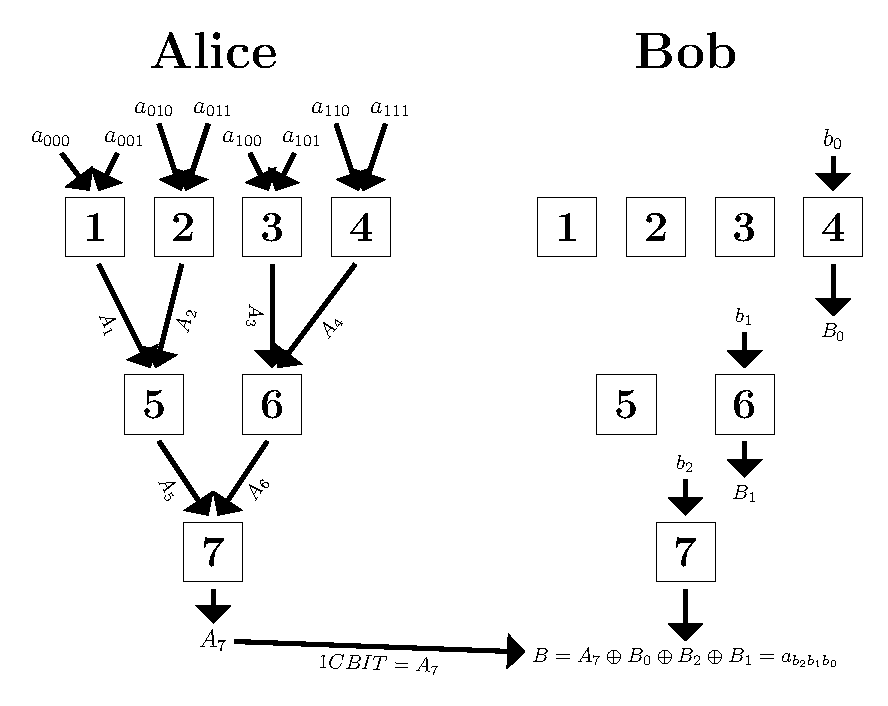
\includegraphics[scale=0.6]{1.eps}
\caption{  The figure demonstrates the use of concatenation of $(2\rightarrow1)$ RB
to form a $(2^{3}\rightarrow 1)$ RB. \textit{RESOURCE: $2^{3}-1=7$ }$(2\rightarrow 1)$
RB. In the figure Bob is trying to learn $a_{101}$ or $a_{111}$.}
\end{figure}
\subsection*{Addition} 
Let us start with a no-signaling $(n\rightarrow 1)$ RB($1$) and a no-signaling $(m\rightarrow 1)$ RB($2$).
We aim at winning the $(n+m\rightarrow 1)$ RAC. The protocol to achieve that is
as follows, \\
\textit{For winning the $(n+m \rightarrow 1)$ box using a no-signaling $(n\rightarrow 1)$ RB, a no-signaling $(m\rightarrow 1)$ RB, an additional  no-signaling $(2\rightarrow 1)$ RB and 1 c-bit of communication:}
Alice has $n$ input bits $a_{0},a_{1}..a_{n-1}$ corresponding to the
no-signaling $(n\rightarrow 1)$ RB($1$) and $m$ inputs bits  $a_{n},a_{n+1}..a_{n+m-1}$
corresponding to the no-signaling $(m\rightarrow 1)$ RB($2$), in total $n+m$ input bits. Alice Obtains a
output bit $A_{1}$ from the no-signaling $(n\rightarrow 1)$ RB($1$) and $A_{2}$ from the no-signaling $(m\rightarrow 1)$
RB($2$).
The {cost} of addition is an additional no-signaling $(2\rightarrow 1)$ RB($3$) whose
input bits are $A_{1}$ and $A_{2}$ and output bit is $A_{3}$. Alice then sends $m=A_{3}$ 
On Bob's end, Bob receives $b\in\{0,1..n-1,n,..n+m-1\}$ and message
$m$. \\
If $0\leq b<n$ then Bob enters $0$ in the no-signaling $(2\rightarrow 1)$ RB(2) and
obtains $B_{3}$ and enters $b$ into no-signaling $(n\rightarrow 1)$ RB($1$) to get
$B_{1}$ and outputs $B=m\oplus B_{1}\oplus B_{3}=a_{b}$.
If $n\leq b\leq n+m-1$ then Bob enters $1$ in the no-signaling $(2\rightarrow1)$ RB(2)
and obtains $B_{3}$ and enters $b$ into no-signaling $(m\rightarrow 1)$ RB($2$) to
get $B_{2}$ and outputs $B=m\oplus B_{2}\oplus B_{3}=a_{b}$.\\
For example winning $(m+n\rightarrow 1)$ RAC using no-signaling $(m\rightarrow 1)$ RB, no-signaling $(n\rightarrow1)$ RB and
a $(2\rightarrow1)$ RB [see FIG. 2].

\begin{figure} 
\includegraphics[scale=0.325]{ADD.pdf}
\caption{  The figure demonstrates the use of addition $(m\rightarrow1)$ RB, $(n\rightarrow 1)$ RB using
a no-signaling $(2\rightarrow1)$ RB.
RB. In the figure Bob is trying to learn $a_b$ for $n\leq b\leq n+m-1$.}
\end{figure}
Finally, protocol for winning the $(n\rightarrow 1)$ RAC using only the no-signaling $(2\rightarrow 1)$ RBs for any $n\in N$. \\
\textit{Protocol for  winning $(n\rightarrow1)$ RAC using no-signaling $(2\rightarrow1)$ RBs:} Any Natural number $n$ can be broken into sum of some discrete powers of $2$, i.e. $n=\sum_{i=0}^{k-1}\alpha_i2^i$ where $\alpha_i\in \{0,1\}$, $i\in\{0,k-2\}$ and $\alpha_{k-1}=1$, $k\in N$ such that $2^{k-1}\leq n< 2^k$. The coefficients $(\alpha_0\alpha_1..\alpha_{k-1})_2$ form the binary representation. We use a variable $count\in N$ and initialize it to $count=0$ for cost calculation given later. Alice receives $n$ input bits and for $i\in \{0,k-1\}$ such that when $\alpha_i=1$, she repeats the following steps,
\begin{enumerate}
\item Use concatenation of $2^i-1$ no-signaling $(2\rightarrow 1)$ RB to construct a $(2^i\rightarrow 1)$ RAC for $i>0$ and for $i=0$ simply take the first input bit $a_0$. Update $count=count+1$ and RB(RIGHT)=$2^i\rightarrow 1$ RB.
\item If $count=1$ Let RB(LEFT)= RB(RIGHT).
\item  If $count>1$: use a no-signaling $(2\rightarrow1)$ RB and ADDTION of $(x\rightarrow1)$ RB(LEFT) and $(y\rightarrow1)$ RB(RIGHT) to form the updated $(x+y\rightarrow 1)$ RB(LEFT).
\end{enumerate}
Alice sends the output of final (bottom most) $(2\rightarrow1)$ RB as the message bit $m$.
Bob receives the message bit $m$ and $b\in\{0,1,2,..,n-1\}$ and outputs $B=a_b$ by following corresponding parts of concatenation and addition. \\
\textit{Cost}: The variable count stores the total number of indexes $i$ such that $_i=1$. concatenation repeated count times uses $(n-count)$ no-signaling $(2\rightarrow1)$ RB. addition is repeated $(count-1)$ each time costing $1$ no-signaling $(2\rightarrow1)$ RB. Finally total cost is $(n-count)+(count-1)=n-1$ no-signaling $(2\rightarrow1)$ RB.
For example winning $(7\rightarrow 1)$ RAC using $(6)$ $(2\rightarrow 1)$ RB [see FIG. 6].
It is to be noted at this point that the protocol given above is just one of many possibilities for simulation of $(n\rightarrow 1)$ RAC using $(n-1)$ $(2\rightarrow 1)$ RB. In particular any construction which forms a fully connected binary tree with no-signaling $(2\rightarrow 1)$ RB as nodes can be used for the simulation $(n\rightarrow 1)$ RAC. In Appendix B we give the proof that $(n-2)$ $(2\rightarrow 1)$ RB (or equivalently PR) cannot simulate $(n\rightarrow 1)$ RAC.  

\textit{Classical and quantum winning probability of $(n\rightarrow1)$ RAC using the above protocol and corresponding bounds on $(2\rightarrow1)$} RAC.\\
One can win the $(n\rightarrow1)$ RAC using $n-1$ no-signaling $(2\rightarrow1)$ RB. Let the quantum and classical winning probabilities over the $(n\rightarrow1)$ RAC be $T_n$ and $C_n$. As the protocol above requires no-signaling $(2\rightarrow1)$ RBs, and  $T_2=\frac{2+\sqrt[]{2}}{4}$ and $C_2=\frac{3}{4}$ are enough to determine $C_n$ and $T_n$ for all $n\in N$ \cite{pawlowski2009information}. Let the winning probability of $(2\rightarrow1)$ RAC be $0<p_2<1$. As an example for $(7\rightarrow1)$ RAC [see FIG. 3] the probability that Bob guesses $a_b$ correctly is $p(B=a_b|b=0)=p_2^2+(1-P^2)^2$,$p(B=a_b|b=1)=(p_2^2+(1-p_2)^2)(p_2)+(1-p_2^2-(1-p_2)^2)(1-p_2)$ and $p(B=a_b|b\in \{1,2,3,4,5,6\})=p(B=a_b|b=1)$. Now Bob's inputs are uniformly distributed, hence $p_7=p(B=a_b)=\frac{p(B=a_b|b=0)+6p(B=a_b|b=1)}{7}$,  $T_7=0.68723$. Similarly, for $(n\rightarrow1)$ RAC for $n\in \{2,..10\}$ the protocol, $C_n$ and $T_n$ are provided in [see FIG. 6]. While $C_n$ are not optimal for $n=2k+1$ \footnote{majority function is not taken into account.}, $T_n$ are numerically close to known optimal values.
\begin{figure*} 
\includegraphics[scale=0.3]{Protocol.pdf}
\caption{ \label{boundMeToTheGround} (Color online)  The figure demonstrates the use of protocol described in Appendix C and $n-1$ no-signaling $(2\rightarrow1)$ RB to win the $(n\rightarrow1)$ RAC for $n\in \{2,3,..10\}$. The C and Q bounds, $C_n$ and $T_n$ are derived recursively using $C_2=0.75$ and $T_2=\frac{2+\sqrt[]{2}}{4}$.  }
\end{figure*}


\section*{Appendix D}
Here we provide the proof for resource inequality in Theorem 5 and consequently the in-equivalence of no-signaling $(2\rightarrow 1,3)$ RB\textsuperscript{2} and $B^3_2$. We give the proof in two parts: 
\begin{enumerate}
\item We shall show that if the $3$it of communication is not used to send the output of Alice's RB $A$ but $B^3_2$-box is obtained, then the channel $\Lambda_3$ is a depolarizing channel: it outputs $z$  or a random $3$it with $\frac{1}{2}$ probability.
\item If the $3$it of communication is used to send $A$ and $B^3_2$-box is obtained, then the capacity of obtainable channel $\Lambda_3$ is upper bounded by $\frac{1}{2}$ $3$it. 
\end{enumerate}
\subsection*{Proof part 1.}
Let $m$ be the message $3$it to be sent to Bob. The goal is to obtain  $B^3_2$-box i.e. $Y=x_y-_3X$ in any case $m=0,1,2$. In general for any $m$ Bob's output is a function of his input $y$ along with the RB $Y=Y(y,b,B)$. Now there are two cases:
\begin{enumerate}
\item \textbf{$A=A'$}: In this case the $B^3_2$-box is obtained by processing a perfect $(2\rightarrow 1,3)$ RAC.
\item \textbf{$A\neq A'$}: In this case the no-signaling $(2\rightarrow 1,3)$ RB\textsuperscript{2} outputs $B$ which does not depend on the work of RAC and hence is useless. Hence Bob's outcome only depends on the input he receives i.e. $Y=Y(y)$. Now we need for  $B^3_2$-box, $Y(y=0)=-_3X$ as $x_0=0$ and $Y(y=1)=x_1-_3X$. Notice Bob can compute $x_1$ using the fact $Y(y=1)-_3Y(y=0)=x_1$. Therefore in this case Bob must know the value of $x_1$.  
\end{enumerate}
Therefore $p_g(x_1|m=m_0)=1$ or $p_g(A|m=m_0)=1$ or both. Where $p_g$ denotes Bob's guessing probability. W.l.o.g. we assume that all three values of $m$ occur with non-zero probability. Bob's simplest strategy (of guessing only one variable, $x_1$ or $A$ for given $m$) can rely on 8 different cases:
\begin{enumerate}
\item $p_g(A|m=0)=1$,$p_g(A|m=1)=1$ and $p_g(A|m=2)=1$
\item $p_g(x_1|m=0)=1$,$p_g(x_1|m=1)=1$ and $p_g(x_1|m=2)=1$
\item $p_g(A|m=0)=1$,$p_g(A|m=1)=1$ and $p_g(x_1|m=2)=1$
\item $p_g(A|m=0)=1$,$p_g(x_1|m=1)=1$ and $p_g(A|m=2)=1$
\item $p_g(x_1|m=0)=1$,$p_g(A|m=1)=1$ and $p_g(A|m=2)=1$
\item $p_g(x_1|m=0)=1$,$p_g(x_1|m=1)=1$ and $p_g(A|m=2)=1$
\item $p_g(x_1|m=0)=1$,$p_g(A|m=1)=1$ and $p_g(x_1|m=2)=1$
\item $p_g(A|m=0)=1$,$p_g(x_1|m=1)=1$ and $p_g(x_1|m=2)=1$
\end{enumerate}
In the third case (equivalently for fourth to eighth cases) Bob makes a perfect guess of $A$ for $m=0,1$ and of $x_1$ for $m=2$. We shall now show by an example (others are analogous), that for the conditions in the third case such a joint probability distribution $p(A,x_1,m)$ cannot exist. Suppose Bob makes a perfect guess, e.g. $A=0$ for $m=0$, $A=1$ for $m=1$ and $x_1=0$. We find that $p(A=2,x_1=1)=0$ and $p(A=2,x_1=2)=0$, which implies the reduced probability distribution $p(A,x_1)$ is no longer randomly distributed, but RB works in a way such that $A$ and $x_1$ are generated independently at random.\\
From the only two possible cases we see that in the first case, $m$ is simply used to send $A$. This case is further dealt with in the Part 2. In the second case the message bit is used to send $x_1$ in this $B^3_2$ box is obtained and the RB serves as an depolarizing $3$it channel with probability $\frac{1}{2}$. $\blacksquare$ 
\subsection*{Proof part 2}
We shall use information theoretic tools to show that if the no-signaling $(2\rightarrow 1,3)$ RB\textsuperscript{2} supplemented with one bit of communication is able to reproduce exactly the $B^3_2$-box and some $3$it channel, then the mutual information of that channel must be bounded by $\frac{1}{2}$ (assuming that Alice's output of RB $A$ is directly inserted into Bob input to the RB i.e. $A=A'$). \\
We shall use the following common assumptions:\\
\textit{Assumptions:} Alice is supplied with two $3$its $x_1,z$, Bob is given a bit $y$. Both are given access to shared random $3$it $s$ such that $x_1,z,y,s$ are mutually independent. Alice generates $X$ and inputs for the RB $a_0,a_1$ from $x_1,z,s$. Similarly Bob generates his input to the RB $b$ from $y,s$. These strategies result in shared joint probability distribution $p(x_1,z,y,s,b,B,X,Y)$ such that $B=a_b$ is obtained from the RAC on Bob's side (as $A$ is always inserted into $A'$) , and $Y$ is generated out of $b,B,s,y$. 
We shall first reformulate Theorem 5 in other words.
Under the aforementioned assumptions, if variables $x_1,y,X,Y$ perfectly reproduce the $B^3_2$-box, there holds:
\begin{equation}\label{main}
I(z:B,b,y,s)\leq \frac{1}{2}
\end{equation}

We shall prove this Theorem in two parts:
\begin{enumerate}
\item First we shall use entropies and correlation to state the fact that to simulate the $B^3_2$-box Bob has to guess perfectly $X$ when $y=0$ and $x_1-_3X$ when $y=1$. 
\item Second we shall show that it is impossible to send more than 1 $3$it through a channel with 1 $3$it capacity. As in our case Alice would like to send both $x_1$ and $z$ which bounds Bob's possible information gain about $z$. 
\end{enumerate}
\begin{mydef2}
Under the aforementioned assumptions, if variables $(x_1,y,X,Y)$ simulate the $B^3_2$-box, there holds:
\begin{eqnarray} \label{ae1}
I(B:x_1-_3X|b,s,y=1)=\nonumber \\H(x_1-_3X|b,s,y=1) \\ \label{ae2}
I(B:X|b,s,y=0)=\nonumber \\ H(X|b,s,y=0) 
\end{eqnarray}
\end{mydef2}
Now in order to perfectly reproduce $B^3_2$-box given $y=0$, he should perfectly guess $X$. On the other hand, given $y=1$ he should perfectly guess $x_1-_3X$. So we must have:
\begin{equation}
J(B,b,s,y=0\rightarrow X)=1 
\end{equation}
and
\begin{equation}
J(B,b,s,y=1\rightarrow x_1-_3X=1 
\end{equation}
where $J(\mathcal{X} \rightarrow \mathcal{Y})=\Sigma_ip(\mathcal{X}=i)\max_j[p(\mathcal{Y}=j|\mathcal{X}=i)]$. Which implies that there must be $max_j[p(X=j|B=l,b=l,y=0,s=i)]=1$, and consequently $H(X|B,b,y=0,s)=0$ which directly leads to (\ref{ae1}). Analogously for (\ref{ae2}). $\blacksquare$\\
\textit{One cannot send more than one $3$it through a single $3$it wire}\\
Here we prove the main argument of Theorem 5. That is, the following Theorem shows the tradeoff between Bob's correlations with $X$ and $x_1-_3X$ and his correlations with $z$. 
\begin{mydef1} \label{At2}
Under aforementioned assumptions, there holds:
\begin{eqnarray} \label{pe1}
\frac{1}{2}I(x_1-_3X:B|b,s,y=1)+\nonumber \\ \frac{1}{2}I(X:B|b,s,y=1)+I(z:B|b,s,y) \leq \nonumber \\ 
\frac{1}{2}I(X:x_1-_3X:z|b,s)+H(B|b,s,y)
\end{eqnarray}
\end{mydef1}
To prove this Theorem we use the following fact:
\begin{eqnarray} \label{te3}
I(S:T|V)+I(T:U|V) \leq 
I(S:U|V)+\nonumber \\ I(T:SU|V)  \equiv I(S:T:U|V)
\end{eqnarray}
The LHS of (\ref{te3}) can be reformulated as, upon fixing $s=i$:
\begin{eqnarray}
\frac{1}{2}I(x_1-_3X:B|b,s=i,y=1)+\nonumber \\ \frac{1}{2}I(X:B|b,s=i,y=1)+I(z:B|b,s=i,y=0) \nonumber \\ I(z:B|b,s=i,y=1)
\end{eqnarray}
Now using (\ref{te3}) to first and third terms and to second and fourth terms, we find that the above quantity is upper bounded by,
\begin{multline}
\frac{1}{2}[I(x_1-_3X:z|b,s=i,y=1)+ \\ I(B:x_1-_3,z|b,s=i,y=1)+ \\ I(X:z|b,s=i,y=0) + \\ I(B:X,z|b,s=i,y=0)]
\end{multline}
Now as $(x_1-_3X,z|s=i)$ is independent from $(y,b|s=i)$, therefore $I(x_1-_3X:z|b,s=i,y=1)=I(x_1-_3X:z|b,s=i)$. And since $(X,z|s=i)$ is independent from $(y,b|s=i)$, there is $I(X:z|b,s=i,y=0)=I(X:z|b,s=i)$. Multiplying these with $p(s=i)$ and summing over values of $s$ we obtain:
\begin{multline}
\frac{1}{2}[I(x_1-_3X:z|b,s)+ \\ I(B:x_1-_3X,z|b,s,y=1)+ \\ I(X:z|b,s) + \\ I(B:X,z|b,s,y=0)]
\end{multline}
We can now use (\ref{te3}) to the first and third terms to obtain the upper bound:
\begin{multline}
\frac{1}{2}[I(x_1-_3X:X|b,s)+ \\ I(z:X,x_1-_3X|b,s)+ \\ I(B:x_1-_3X,z|b,s,y=1) + \\ I(B:X,z|b,s,y=0)]
\end{multline}
Now $I(x_1-_3X:X|b,s)+I(z:X,x_1-_3X|b,s)=I(z:X:x_1-_3X|b,s)$. Also 
$\frac{1}{2}[I(B:x_1-_3X,z|b,s,y=1) +  I(B:X,z|b,s,y=0)]\leq H(B|b,s,y)$, and (\ref{pe1}) follows. $\blacksquare$\\
Finally, we shall proof the inequality (\ref{main}). From the chain rule: $I(z:B,b,s,y)=I(z:y,s,b)+I(z:B|y,s,b)$ but $I(z:y,s)=I(z:y,b,s)=0$ ($b=b(y,s)$). Hence \ref{main} can be reformulated as:
\begin{equation} \label{main2}
I(z:B|s,b,y)\leq \frac{1}{2}
\end{equation}
To prove (\ref{main2}) we shall reformulate (\ref{pe1}) using (\ref{ae1}) and (\ref{ae2}):
\begin{multline}
\frac{1}{2}[H(X|b,s,y=0)+H(x_1-_3X|b,s,y=1)]+\\I(z:B|b,s,y) \leq \frac{1}{2}[H(X|b,s)+H(x_1-_3X|b,s)+\\H(z|b,s)-H(X,x_1-_3X,z|b,s)]+\\H(B|b,s,y)
\end{multline}
Now as $(X|s=i)$  and $(x_1-_3X|s=i)$ are independent from $(b,y|s=i)$, we have for each $i$ that $H(X|b,s=i,y=0)=H(X|b,s=i)$ and $H(x_1-_3X|b,s=i,y=1)=H(x_1-_3X|b,s=i)$. And because for some fixed $s=i$, $z$ is independent of $b$, we have $H(z|b,s=i)=H(z|s=i)$. Averaging these equalities over $p(s=i)$ we obtain:
\begin{multline}
I(z:B|y,b,s) \leq \\ \frac{1}{2}[H(z|s)-H(X,x_1-_3X,z|b,s)]+H(B|y,s,b)
\end{multline}
Now $z$ is independent of from $s$, $H(z|s)=H(z|s)=1$. And $H(X,x_1-_3X,z|s)=H(X,x_1,z|b,s)$ as we can add $X$ to $x_1-_3X$. Using the data processing inequality and the independence of $s$ form $(x,z)$ we get, $H(z,X,x_1|s)\geq H(z,x_1|s)=H(z,x_1)=2$. Hence the first two terms are upper bounded by $-\frac{1}{2}$. The last term trivially upper bounded by $1$, which results in $\frac{1}{2}$ proving (\ref{main2}) $\blacksquare$.
